
%% bare_jrnl.tex
%% V1.3
%% 2007/01/11
%% by Michael Shell
%% see http://www.michaelshell.org/
%% for current contact information.
%%
%% This is a skeleton file demonstrating the use of IEEEtran.cls
%% (requires IEEEtran.cls version 1.7 or later) with an IEEE journal paper.
%%
%% Support sites:
%% http://www.michaelshell.org/tex/ieeetran/
%% http://www.ctan.org/tex-archive/macros/latex/contrib/IEEEtran/
%% and
%% http://www.ieee.org/



% *** Authors should verify (and, if needed, correct) their LaTeX system  ***
% *** with the testflow diagnostic prior to trusting their LaTeX platform ***
% *** with production work. IEEE's font choices can trigger bugs that do  ***
% *** not appear when using other class files.                            ***
% The testflow support page is at:
% http://www.michaelshell.org/tex/testflow/


%%*************************************************************************
%% Legal Notice:
%% This code is offered as-is without any warranty either expressed or
%% implied; without even the implied warranty of MERCHANTABILITY or
%% FITNESS FOR A PARTICULAR PURPOSE!
%% User assumes all risk.
%% In no event shall IEEE or any contributor to this code be liable for
%% any damages or losses, including, but not limited to, incidental,
%% consequential, or any other damages, resulting from the use or misuse
%% of any information contained here.
%%
%% All comments are the opinions of their respective authors and are not
%% necessarily endorsed by the IEEE.
%%
%% This work is distributed under the LaTeX Project Public License (LPPL)
%% ( http://www.latex-project.org/ ) version 1.3, and may be freely used,
%% distributed and modified. A copy of the LPPL, version 1.3, is included
%% in the base LaTeX documentation of all distributions of LaTeX released
%% 2003/12/01 or later.
%% Retain all contribution notices and credits.
%% ** Modified files should be clearly indicated as such, including  **
%% ** renaming them and changing author support contact information. **
%%
%% File list of work: IEEEtran.cls, IEEEtran_HOWTO.pdf, bare_adv.tex,
%%                    bare_conf.tex, bare_jrnl.tex, bare_jrnl_compsoc.tex
%%*************************************************************************

% Note that the a4paper option is mainly intended so that authors in
% countries using A4 can easily print to A4 and see how their papers will
% look in print - the typesetting of the document will not typically be
% affected with changes in paper size (but the bottom and side margins will).
% Use the testflow package mentioned above to verify correct handling of
% both paper sizes by the user's LaTeX system.
%
% Also note that the "draftcls" or "draftclsnofoot", not "draft", option
% should be used if it is desired that the figures are to be displayed in
% draft mode.
%
\documentclass[journal]{IEEEtran}

\newtheorem{definition}{Definition}
\newtheorem{proposition}{Proposition}
\newtheorem{theorem}{Theorem}
\newtheorem{remark}{Remark}

% to add comments in different colors (added by Azadeh)
\usepackage[usenames]{color}
\usepackage{lscape}
\usepackage{soul}
\newcommand{\blue}[1]{{\color{blue} #1}}
\newcommand{\red}[1]{{\color{red} #1}}
\newcommand{\black}[1]{{\color{black} #1}}

\newcommand{\Az}[1]{{\color{blue}{#1}}}
%\newcommand{\AzCom}[1]{{\it \color{magenta} [#1]}}
\newcommand{\AzCom}[1]{}
%\newcommand{\AzDel}[1]{{\color{red} \st{#1}}}
%\newcommand{\AzDel}[1]{{\color{Gray}{\{#1\}}}}
\newcommand{\AzDel}[1]{}

\newdimen\snellbaselineskip
\newdimen\snellskip
\snellskip=1.5ex
\snellbaselineskip=\baselineskip
\def\srule{\omit\kern.5em\vrule\kern-.5em}
\newbox\bigstrutbox
\setbox\bigstrutbox=\hbox{\vrule height14.5pt depth9.5pt width0pt}
\def\bigstrut{\relax\ifmmode\copy\bigstrutbox\else\unhcopy\bigstrutbox\fi}
\def\middlehrule#1#2{\noalign{\kern-\snellbaselineskip\kern\snellskip}
&\multispan#1\strut\hrulefill
&\omit\hbox to.5em{\hrulefill}\vrule
height \snellskip\kern-.5em&\multispan#2\hrulefill\cr}


\makeatletter
\def\bordermatrix#1{\begingroup \m@th
  \@tempdima 8.75\p@
  \setbox\z@\vbox{%
    \def\cr{\crcr\noalign{\kern2\p@\global\let\cr\endline}}%
    \ialign{$##$\hfil\kern2\p@\kern\@tempdima&\thinspace\hfil$##$\hfil
      &&\quad\hfil$##$\hfil\crcr
      \omit\strut\hfil\crcr\noalign{\kern-\snellbaselineskip}%
      #1\crcr\omit\strut\cr}}%
  \setbox\tw@\vbox{\unvcopy\z@\global\setbox\@ne\lastbox}%
  \setbox\tw@\hbox{\unhbox\@ne\unskip\global\setbox\@ne\lastbox}%
  \setbox\tw@\hbox{$\kern\wd\@ne\kern-\@tempdima\left(\kern-\wd\@ne
    \global\setbox\@ne\vbox{\box\@ne\kern2\p@}%
    \vcenter{\kern-\ht\@ne\unvbox\z@\kern-\snellbaselineskip}\,\right)$}%
  \null\;\vbox{\kern\ht\@ne\box\tw@}\endgroup}
\makeatletter

\makeatletter
\def\bordermatrix#1{\begingroup \m@th
  \@tempdima 8.75\p@
  \setbox\z@\vbox{%
    \def\cr{\crcr\noalign{\kern2\p@\global\let\cr\endline}}%
    \ialign{$##$\hfil\kern2\p@\kern\@tempdima&\thinspace\hfil$##$\hfil
      &&\quad\hfil$##$\hfil\crcr
      \omit\strut\hfil\crcr\noalign{\kern-\snellbaselineskip}%
      #1\crcr\omit\strut\cr}}%
  \setbox\tw@\vbox{\unvcopy\z@\global\setbox\@ne\lastbox}%
  \setbox\tw@\hbox{\unhbox\@ne\unskip\global\setbox\@ne\lastbox}%
  \setbox\tw@\hbox{$\kern\wd\@ne\kern-\@tempdima\left(\kern-\wd\@ne
    \global\setbox\@ne\vbox{\box\@ne\kern2\p@}%
    \vcenter{\kern-\ht\@ne\unvbox\z@\kern-\snellbaselineskip}\,\right)$}%
  \null\;\vbox{\kern\ht\@ne\box\tw@}\endgroup}
\makeatletter

%
% If IEEEtran.cls has not been installed into the LaTeX system files,
% manually specify the path to it like:
% \documentclass[journal]{../sty/IEEEtran}





% Some very useful LaTeX packages include:
% (uncomment the ones you want to load)


% *** MISC UTILITY PACKAGES ***
%
%\usepackage{ifpdf}
% Heiko Oberdiek's ifpdf.sty is very useful if you need conditional
% compilation based on whether the output is pdf or dvi.
% usage:
% \ifpdf
%   % pdf code
% \else
%   % dvi code
% \fi
% The latest version of ifpdf.sty can be obtained from:
% http://www.ctan.org/tex-archive/macros/latex/contrib/oberdiek/
% Also, note that IEEEtran.cls V1.7 and later provides a builtin
% \ifCLASSINFOpdf conditional that works the same way.
% When switching from latex to pdflatex and vice-versa, the compiler may
% have to be run twice to clear warning/error messages.






% *** CITATION PACKAGES ***
%
\usepackage{cite}
% cite.sty was written by Donald Arseneau
% V1.6 and later of IEEEtran pre-defines the format of the cite.sty package
% \cite{} output to follow that of IEEE. Loading the cite package will
% result in citation numbers being automatically sorted and properly
% "compressed/ranged". e.g., [1], [9], [2], [7], [5], [6] without using
% cite.sty will become [1], [2], [5]--[7], [9] using cite.sty. cite.sty's
% \cite will automatically add leading space, if needed. Use cite.sty's
% noadjust option (cite.sty V3.8 and later) if you want to turn this off.
% cite.sty is already installed on most LaTeX systems. Be sure and use
% version 4.0 (2003-05-27) and later if using hyperref.sty. cite.sty does
% not currently provide for hyperlinked citations.
% The latest version can be obtained at:
% http://www.ctan.org/tex-archive/macros/latex/contrib/cite/
% The documentation is contained in the cite.sty file itself.






% *** GRAPHICS RELATED PACKAGES ***
%
\ifCLASSINFOpdf
  % \usepackage[pdftex]{graphicx}
  % declare the path(s) where your graphic files are
  % \graphicspath{{../pdf/}{../jpeg/}}
  % and their extensions so you won't have to specify these with
  % every instance of \includegraphics
  % \DeclareGraphicsExtensions{.pdf,.jpeg,.png}
\else
  % or other class option (dvipsone, dvipdf, if not using dvips). graphicx
  % will default to the driver specified in the system graphics.cfg if no
  % driver is specified.
  \usepackage[dvips]{graphicx}
  % declare the path(s) where your graphic files are
  % \graphicspath{{../eps/}}
  % and their extensions so you won't have to specify these with
  % every instance of \includegraphics
  \DeclareGraphicsExtensions{.eps}
\fi
% graphicx was written by David Carlisle and Sebastian Rahtz. It is
% required if you want graphics, photos, etc. graphicx.sty is already
% installed on most LaTeX systems. The latest version and documentation can
% be obtained at:
% http://www.ctan.org/tex-archive/macros/latex/required/graphics/
% Another good source of documentation is "Using Imported Graphics in
% LaTeX2e" by Keith Reckdahl which can be found as epslatex.ps or
% epslatex.pdf at: http://www.ctan.org/tex-archive/info/
%
% latex, and pdflatex in dvi mode, support graphics in encapsulated
% postscript (.eps) format. pdflatex in pdf mode supports graphics
% in .pdf, .jpeg, .png and .mps (metapost) formats. Users should ensure
% that all non-photo figures use a vector format (.eps, .pdf, .mps) and
% not a bitmapped formats (.jpeg, .png). IEEE frowns on bitmapped formats
% which can result in "jaggedy"/blurry rendering of lines and letters as
% well as large increases in file sizes.
%
% You can find documentation about the pdfTeX application at:
% http://www.tug.org/applications/pdftex





% *** MATH PACKAGES ***
%
\usepackage[cmex10]{amsmath}
% A popular package from the American Mathematical Society that provides
% many useful and powerful commands for dealing with mathematics. If using
% it, be sure to load this package with the cmex10 option to ensure that
% only type 1 fonts will utilized at all point sizes. Without this option,
% it is possible that some math symbols, particularly those within
% footnotes, will be rendered in bitmap form which will result in a
% document that can not be IEEE Xplore compliant!
%
% Also, note that the amsmath package sets \interdisplaylinepenalty to 10000
% thus preventing page breaks from occurring within multiline equations. Use:
%\interdisplaylinepenalty=2500
% after loading amsmath to restore such page breaks as IEEEtran.cls normally
% does. amsmath.sty is already installed on most LaTeX systems. The latest
% version and documentation can be obtained at:
% http://www.ctan.org/tex-archive/macros/latex/required/amslatex/math/

\usepackage{amssymb}
\usepackage{amsfonts}




% *** SPECIALIZED LIST PACKAGES ***
%
%\usepackage{algorithmic}
% algorithmic.sty was written by Peter Williams and Rogerio Brito.
% This package provides an algorithmic environment fo describing algorithms.
% You can use the algorithmic environment in-text or within a figure
% environment to provide for a floating algorithm. Do NOT use the algorithm
% floating environment provided by algorithm.sty (by the same authors) or
% algorithm2e.sty (by Christophe Fiorio) as IEEE does not use dedicated
% algorithm float types and packages that provide these will not provide
% correct IEEE style captions. The latest version and documentation of
% algorithmic.sty can be obtained at:
% http://www.ctan.org/tex-archive/macros/latex/contrib/algorithms/
% There is also a support site at:
% http://algorithms.berlios.de/index.html
% Also of interest may be the (relatively newer and more customizable)
% algorithmicx.sty package by Szasz Janos:
% http://www.ctan.org/tex-archive/macros/latex/contrib/algorithmicx/




% *** ALIGNMENT PACKAGES ***
%
%\usepackage{array}
% Frank Mittelbach's and David Carlisle's array.sty patches and improves
% the standard LaTeX2e array and tabular environments to provide better
% appearance and additional user controls. As the default LaTeX2e table
% generation code is lacking to the point of almost being broken with
% respect to the quality of the end results, all users are strongly
% advised to use an enhanced (at the very least that provided by array.sty)
% set of table tools. array.sty is already installed on most systems. The
% latest version and documentation can be obtained at:
% http://www.ctan.org/tex-archive/macros/latex/required/tools/


%\usepackage{mdwmath}
%\usepackage{mdwtab}
% Also highly recommended is Mark Wooding's extremely powerful MDW tools,
% especially mdwmath.sty and mdwtab.sty which are used to format equations
% and tables, respectively. The MDWtools set is already installed on most
% LaTeX systems. The lastest version and documentation is available at:
% http://www.ctan.org/tex-archive/macros/latex/contrib/mdwtools/


% IEEEtran contains the IEEEeqnarray family of commands that can be used to
% generate multiline equations as well as matrices, tables, etc., of high
% quality.


%\usepackage{eqparbox}
% Also of notable interest is Scott Pakin's eqparbox package for creating
% (automatically sized) equal width boxes - aka "natural width parboxes".
% Available at:
% http://www.ctan.org/tex-archive/macros/latex/contrib/eqparbox/





% *** SUBFIGURE PACKAGES ***
%\usepackage[tight,footnotesize]{subfigure}
% subfigure.sty was written by Steven Douglas Cochran. This package makes it
% easy to put subfigures in your figures. e.g., "Figure 1a and 1b". For IEEE
% work, it is a good idea to load it with the tight package option to reduce
% the amount of white space around the subfigures. subfigure.sty is already
% installed on most LaTeX systems. The latest version and documentation can
% be obtained at:
% http://www.ctan.org/tex-archive/obsolete/macros/latex/contrib/subfigure/
% subfigure.sty has been superceeded by subfig.sty.



%\usepackage[caption=false]{caption}
%\usepackage[font=footnotesize]{subfig}
% subfig.sty, also written by Steven Douglas Cochran, is the modern
% replacement for subfigure.sty. However, subfig.sty requires and
% automatically loads Axel Sommerfeldt's caption.sty which will override
% IEEEtran.cls handling of captions and this will result in nonIEEE style
% figure/table captions. To prevent this problem, be sure and preload
% caption.sty with its "caption=false" package option. This is will preserve
% IEEEtran.cls handing of captions. Version 1.3 (2005/06/28) and later
% (recommended due to many improvements over 1.2) of subfig.sty supports
% the caption=false option directly:
%\usepackage[caption=false,font=footnotesize]{subfig}
%
% The latest version and documentation can be obtained at:
% http://www.ctan.org/tex-archive/macros/latex/contrib/subfig/
% The latest version and documentation of caption.sty can be obtained at:
% http://www.ctan.org/tex-archive/macros/latex/contrib/caption/




% *** FLOAT PACKAGES ***
%
%\usepackage{fixltx2e}
% fixltx2e, the successor to the earlier fix2col.sty, was written by
% Frank Mittelbach and David Carlisle. This package corrects a few problems
% in the LaTeX2e kernel, the most notable of which is that in current
% LaTeX2e releases, the ordering of single and double column floats is not
% guaranteed to be preserved. Thus, an unpatched LaTeX2e can allow a
% single column figure to be placed prior to an earlier double column
% figure. The latest version and documentation can be found at:
% http://www.ctan.org/tex-archive/macros/latex/base/



%\usepackage{stfloats}
% stfloats.sty was written by Sigitas Tolusis. This package gives LaTeX2e
% the ability to do double column floats at the bottom of the page as well
% as the top. (e.g., "\begin{figure*}[!b]" is not normally possible in
% LaTeX2e). It also provides a command:
%\fnbelowfloat
% to enable the placement of footnotes below bottom floats (the standard
% LaTeX2e kernel puts them above bottom floats). This is an invasive package
% which rewrites many portions of the LaTeX2e float routines. It may not work
% with other packages that modify the LaTeX2e float routines. The latest
% version and documentation can be obtained at:
% http://www.ctan.org/tex-archive/macros/latex/contrib/sttools/
% Documentation is contained in the stfloats.sty comments as well as in the
% presfull.pdf file. Do not use the stfloats baselinefloat ability as IEEE
% does not allow \baselineskip to stretch. Authors submitting work to the
% IEEE should note that IEEE rarely uses double column equations and
% that authors should try to avoid such use. Do not be tempted to use the
% cuted.sty or midfloat.sty packages (also by Sigitas Tolusis) as IEEE does
% not format its papers in such ways.


%\ifCLASSOPTIONcaptionsoff
%  \usepackage[nomarkers]{endfloat}
% \let\MYoriglatexcaption\caption
% \renewcommand{\caption}[2][\relax]{\MYoriglatexcaption[#2]{#2}}
%\fi
% endfloat.sty was written by James Darrell McCauley and Jeff Goldberg.
% This package may be useful when used in conjunction with IEEEtran.cls'
% captionsoff option. Some IEEE journals/societies require that submissions
% have lists of figures/tables at the end of the paper and that
% figures/tables without any captions are placed on a page by themselves at
% the end of the document. If needed, the draftcls IEEEtran class option or
% \CLASSINPUTbaselinestretch interface can be used to increase the line
% spacing as well. Be sure and use the nomarkers option of endfloat to
% prevent endfloat from "marking" where the figures would have been placed
% in the text. The two hack lines of code above are a slight modification of
% that suggested by in the endfloat docs (section 8.3.1) to ensure that
% the full captions always appear in the list of figures/tables - even if
% the user used the short optional argument of \caption[]{}.
% IEEE papers do not typically make use of \caption[]'s optional argument,
% so this should not be an issue. A similar trick can be used to disable
% captions of packages such as subfig.sty that lack options to turn off
% the subcaptions:
% For subfig.sty:
% \let\MYorigsubfloat\subfloat
% \renewcommand{\subfloat}[2][\relax]{\MYorigsubfloat[]{#2}}
% For subfigure.sty:
% \let\MYorigsubfigure\subfigure
% \renewcommand{\subfigure}[2][\relax]{\MYorigsubfigure[]{#2}}
% However, the above trick will not work if both optional arguments of
% the \subfloat/subfig command are used. Furthermore, there needs to be a
% description of each subfigure *somewhere* and endfloat does not add
% subfigure captions to its list of figures. Thus, the best approach is to
% avoid the use of subfigure captions (many IEEE journals avoid them anyway)
% and instead reference/explain all the subfigures within the main caption.
% The latest version of endfloat.sty and its documentation can obtained at:
% http://www.ctan.org/tex-archive/macros/latex/contrib/endfloat/
%
% The IEEEtran \ifCLASSOPTIONcaptionsoff conditional can also be used
% later in the document, say, to conditionally put the References on a
% page by themselves.





% *** PDF, URL AND HYPERLINK PACKAGES ***
%
\usepackage{url}
% url.sty was written by Donald Arseneau. It provides better support for
% handling and breaking URLs. url.sty is already installed on most LaTeX
% systems. The latest version can be obtained at:
% http://www.ctan.org/tex-archive/macros/latex/contrib/misc/
% Read the url.sty source comments for usage information. Basically,
% \url{my_url_here}.

\usepackage{psfrag}



% *** Do not adjust lengths that control margins, column widths, etc. ***
% *** Do not use packages that alter fonts (such as pslatex).         ***
% There should be no need to do such things with IEEEtran.cls V1.6 and later.
% (Unless specifically asked to do so by the journal or conference you plan
% to submit to, of course. )


% correct bad hyphenation here

\def\Abf{{\mathbf{A}}}
\def\Pbf{{\mathbf{P}}}
\newcommand{\pr}[1]{\Pr \left\{#1\right\}}
\hyphenation{op-tical net-works semi-conduc-tor}


\begin{document}
%
% paper title
% can use linebreaks \\ within to get better formatting as desired
\title{Address Reuse in the Bitcoin Network}
%
%
% author names and IEEE memberships
% note positions of commas and nonbreaking spaces ( ~ ) LaTeX will not break
% a structure at a ~ so this keeps an author's name from being broken across
% two lines.
% use \thanks{} to gain access to the first footnote area
% a separate \thanks must be used for each paragraph as LaTeX2e's \thanks
% was not built to handle multiple paragraphs
%

\author{Name~Surname, %~\IEEEmembership{Member,~IEEE,}
        Name~Surname, %~\IEEEmembership{Fellow,~OSA,}
        Name~Surname, \IEEEmembership{Member, IEEE,}
        Name~Surname, %~\IEEEmembership{Fellow,~OSA,}
        and~Name~Surname,~\IEEEmembership{Senior~Member,~IEEE}% <-this % stops a space
\thanks{The authors are with Universitat Pompeu Fabra.
Roc Boronat 138, 08018 Barcelona, Catalunya, Spain.
E-mail: jaume.barcelo@upf.edu
This paper has been submitted to an IEEE journal.
}
}

% note the % following the last \IEEEmembership and also \thanks -
% these prevent an unwanted space from occurring between the last author name
% and the end of the author line. i.e., if you had this:
%
% \author{....lastname \thanks{...} \thanks{...} }
%                     ^------------^------------^----Do not want these spaces!
%
% a space would be appended to the last name and could cause every name on that
% line to be shifted left slightly. This is one of those "LaTeX things". For
% instance, "\textbf{A} \textbf{B}" will typeset as "A B" not "AB". To get
% "AB" then you have to do: "\textbf{A}\textbf{B}"
% \thanks is no different in this regard, so shield the last } of each \thanks
% that ends a line with a % and do not let a space in before the next \thanks.
% Spaces after \IEEEmembership other than the last one are OK (and needed) as
% you are supposed to have spaces between the names. For what it is worth,
% this is a minor point as most people would not even notice if the said evil
% space somehow managed to creep in.



% The paper headers
\markboth{Journal of \LaTeX\ Class Files,~Vol.~6, No.~1, January~2007}%
{Shell \MakeLowercase{\textit{et al.}}: Bare Demo of IEEEtran.cls for Journals}
% The only time the second header will appear is for the odd numbered pages
% after the title page when using the twoside option.
%
% *** Note that you probably will NOT want to include the author's ***
% *** name in the headers of peer review papers.                   ***
% You can use \ifCLASSOPTIONpeerreview for conditional compilation here if
% you desire.




% If you want to put a publisher's ID mark on the page you can do it like
% this:
%\IEEEpubid{0000--0000/00\$00.00~\copyright~2007 IEEE}
% Remember, if you use this you must call \IEEEpubidadjcol in the second
% column for its text to clear the IEEEpubid mark.



% use for special paper notices
%\IEEEspecialpapernotice{(Invited Paper)}




% make the title area
\maketitle


\begin{abstract}
Bitcoin is a peer-to-peer electronic cash system that maintains a public ledger with all transactions.
The public availability of this information has implications for the privacy of the users.
The public ledger consists of transactions that transfer funds from a set of inputs to a set of output addresses.
As long as those addresses cannot be linked to their owners, privacy is preserved.
The linking of addresses to owners results in privacy leaks.
The possibilities of linking addresses to owners are multiplied when addresses are used to receive funds more than once.
In this work we privacy-leaking effects of address reuse and gather statistics of address reuse in the Bitcoin network.
\end{abstract}
% IEEEtran.cls defaults to using nonbold math in the Abstract.
% This preserves the distinction between vectors and scalars. However,
% if the journal you are submitting to favors bold math in the abstract,
% then you can use LaTeX's standard command \boldmath at the very start
% of the abstract to achieve this. Many IEEE journals frown on math
% in the abstract anyway.

% Note that keywords are not normally used for peerreview papers.
\begin{IEEEkeywords}
Bitcoin, cryptocurrency, privacy, address reuse
\end{IEEEkeywords}






% For peer review papers, you can put extra information on the cover
% page as needed:
% \ifCLASSOPTIONpeerreview
% \begin{center} \bfseries EDICS Category: 3-BBND \end{center}
% \fi
%
% For peerreview papers, this IEEEtran command inserts a page break and
% creates the second title. It will be ignored for other modes.
\IEEEpeerreviewmaketitle



\section{Introduction}
% The very first letter is a 2 line initial drop letter followed
% by the rest of the first word in caps.
%
% form to use if the first word consists of a single letter:
% \IEEEPARstart{A}{demo} file is ....
%
% form to use if you need the single drop letter followed by
% normal text (unknown if ever used by IEEE):
% \IEEEPARstart{A}{}demo file is ....
%
% Some journals put the first two words in caps:
% \IEEEPARstart{T}{his demo} file is ....
%
% Here we have the typical use of a "T" for an initial drop letter
% and "HIS" in caps to complete the first word.

% \IEEEPARstart{I}{n} this paper we discuss a family of protocols that can be used for radio resource assignment in wireless networks.
% The problem of assigning resources in a distributed fashion is defined as a Decentralized Constraint Satisfaction (DCS) problem \cite{duffy2011dcs}.
% We consider a particular solver for this family of problems that works iteratively, in several rounds, to find a solution to the problem.

% The solver performs a stochastic search until it converges to a solution.
% You must have at least 2 lines in the paragraph with the drop letter
% (should never be an issue)

\IEEEPARstart{B}{itcoin} is a peer-to-peer electronic cash system \cite{nakamoto2008bpp} that maintains a public ledger with all transactions.
All the transactions need to be available to the peer-to-peer network that guarantees the security of the system.
Any full node of the network stores in a database all the transactions in the history of Bitcoin.
This database is typically referred to as the \emph{Blockchain}.

With traditional cash, there is no public record of all the transactions.
And the traditional banking system keeps the transactions of their customers private.
Therefore, the privacy that Bitcoin offers to its users is a matter study.
Ideally, any new payment system should offer privacy guarantees at least as good as traditional systems.

Bitcoin are sent to Bitcoin addresses, and both the Bitcoin community and previous research studies agree that address reuse is in general a bad practice.
It is recommended to generate a new address for each payment to be received.
This addresses that are used only ones are called disposable addresses.

In this paper we first review the basic elements of the Bitcoin system necessary for the subsequent discussion.
Then we discuss the necessity of avoiding address re-use to prevent unnecessary privacy leakage.
After that, we analyze the Blockchain to determine to which extend address reuse occurs in the Bitcoin community.
Disposable addresses do not offer total protection against privacy leakage and we detail the remaining risks as well as possible solutions.
Finally, we conclude.

\section{Address Reuse}

\subsection{Basic Bitcoin Elements}

Bitcoin is a protocol, a network, and an Internet currency unit.
We capitalize the word when we refer to either the protocol or the network.

Transactions are a fundamental element of Bicoin.
Payments require transactions, and these transactions are shared with the network and securely stored in the Blockchain.
Each transaction consumes some inputs and creates some outputs.
The inputs and outputs are worth bitcoins, and for a regular transaction to be valid the total value of the outputs must not exceed the total amount of the inputs.

The outputs of one transaction can be used as inputs of other transactions.
Critically, each output can be used only once.
The words consumed or spent are common synonyms of used in this context.
The idea is that each output can be spent only once just as we can spend our money only once.
The network does not accept transactions that try to spend outputs that have been spent before.

Another important element of Bitcoin are public/private asymmetric cryptographical keys.
The public key is hashed and coded with some redundancy into base58 addresses.
These addresses are alphanumeric chains that can be used to receive funds.
The outputs of a transaction can be send to an address, which is simply a convenient representation of a public key.

In order to spend an output, it is then necessary to offer proof of ownership of the address and, consequently, of the output.
This proof is the evidence of knowledge of the private key corresponding to the address.
A user willing to spend an output sent to a given address must provide the public address that hashes to the address and a valid signature.
The signature can be generated only by the owner of the private key.

There is no limit in Bitcoin regarding the number of outputs that can be send to a Bitcoin address.
The owner of the private key will be able to spend all of those outputs once.
Another particularity of bitcoin is that there is no practical limit of the number of addresses that can be generated.
There are $2^{160}$ possible addresses because they are generated using RIPE-MD160.
This makes it possible for users to generate new (disposable) addresses for each incoming payment.

A particular form of outputs which is relevant to the discussion later in this work are \emph{change} outputs.
A user willing to send a Bitcoin payment needs to combine in a transaction a number of inputs of value equal or larger than the desired payment.
If the value of the inputs is larger than the output, it is likely that the sending part does not want to loose the difference, also called change.
In order to keep the change, the payer creates a transaction with inputs exceeding the payment value and two outputs: the actual payment and the change.
The payment is sent to the payee and the change is sent to an address controlled by the payer.

It is a common and recommended practice that the amount of the inputs is slightly higher than the value of the outputs.
This small difference is called a \emph{fee} and it is kept by the peers that contributed to the security of the network.



\subsection{The Temptation}

The temptation exists of using Bitcoin addresses just like regular bank accounts numbers.
As addresses are used to receive payments, technically speaking only once is needed.
We can use the same address to receive all our payments, just like we can use a single bank account to receive all our payments.
Obviously, in this case, we will also use the same address for all the payments which is in agreement with the bank account parallelism. 

The difference is that our bank account transactions and balance are kept private by our bank.
In contrast, all the transactions and balances in Bitcoin are publicly available to anyone with internet access.
We could retain our privacy if we were able to keep our Bitcoin.
However, each time that we make a transaction, the other transacting party learns our address and therefore all our transaction history.

Address reuse is discouraged in the original Bitcoin paper \cite{nakamoto2008bpp}.

\subsection{Address Reuse in the Blockchain}

Even though address reuse might have worrying consequences, the fact is that we can find address reuse in the public record of all Bitcon transactions.
All transactions are securely stored in the Blockchain.
We use Obelisk and Libbitcoin to download and query the Blockchain for evidence of address reuse.
Both Obelisk and Libbitcoin are open source projects under heavy development. 
Our source code to generate the data and the plots presented in the paper is also available in github\footnote{http://github.com}.
We sweep all the transactions in the Bitcoin history and for every address we count how many times it appears as an output of a transaction.

Some statistics of the distribution are presented in Table~\ref{tab:address-reuse}.
A histogram of the data is presented in Fig.~\ref{fig:address-reuse}.
For readability reasons, we can only show the first 100 positions of the histogram.
The distribution has a long tail and some addresses are used over one million times.




\subsection{Wikileaks Privacy Leakage}

Wikileaks funding campaign is an example of address re-use.
At the time of this writing, Wikileak's donation webpage offers by default a re-used address.
It also offers the donors the possibility of generating a new (one-time) address by simply clicking a button.
The public address makes it possible for everyone to inspect all the details of the transactions involving that address.
A Blockchain explorer website (such as \texttt{blockchain.info}) can be used to browse all those details.
At the time of this writing, Wikileak's public address has received over 3,854 bitcoins in 2216 transactions.
The source addresses for each transaction are also public.

Wikileaks address reuse can unintendedly leak donor's privacy unless they are very cautious.
Any payer can check if the output of the payment is later spend in a transaction to Wikileaks.
If this is the case, the payer know that the payee is also a Wikileaks donor.

There are more sophisticated techniques that we review later in this paper that can result in increased privacy leakage taking advantage of the widespread use of Bitcoin \emph{wallets} and \emph{change addresses}.

\begin{table}[!t]
% increase table row spacing, adjust to taste
\renewcommand{\arraystretch}{1.3}
% if using array.sty, it might be a good idea to tweak the value of
% \extrarowheight as needed to properly center the text within the cells
\caption{Address Re-use Statistics}
\label{tab:address-reuse}
\centering
%% Some packages, such as MDW tools, offer better commands for making tables
%% than the plain LaTeX2e tabular which is used here.
\begin{tabular}{|cc|}
\hline
Mean & 3.18\\
Min & 1\\
25th perc. & 1 \\
50th perc. & 1 \\
75th perc. & 1 \\
Max & 1,238,931\\
Number of addresses & 12,963,199 \\
Number of uses & 41,244,997 \\
Addresses used once & 10,476,899 \\
Addressed used twice & 1,397,373\\
Used over 100 times & 25,004 \\
\hline
\end{tabular}
\end{table}

\begin{figure}[!t]
\centering
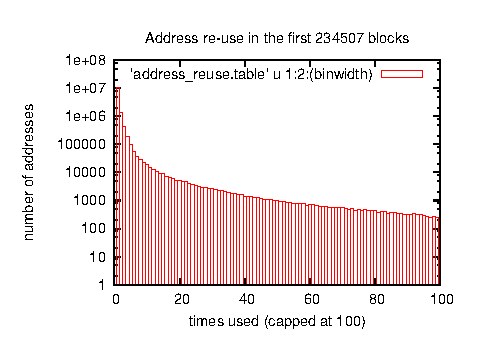
\includegraphics[width=\linewidth]{figures/address-reuse.eps}
\caption{Number of addresses for re-use factor from 1 to 100. Note the log scale.}
\label{fig:address-reuse}
\end{figure}

\subsection{Bitcoin Wallets}

From the previous section it should be clear that address reuse has negative consequences to the user's privacy.
A partial solution to Bitcoin's privacy weaknesses is the use of disposable addresses.
Disposable addresses are used only once and therefore make it more difficult to link different transactions to the same user.

The reference Bitcoin peer implementation, \emph{bitcoind} and many other software packages make it possible for th Bitcoin user to comfortably handle a large number of addresses.
The software that takes care of Bitcoin addresses is called a Bitcoin wallet.
This software generates as many addresses as needed.
Some of these addresses are used for receiving payments while others are used to receive change outputs.
The software does not reuse change addresses and therefore, if the user is cautious enough to avoid address reuse for payment reception, addresses are used a single time to receive funds.

The software wallet also adds the funds available in all the addresses to present a total balance to the user.
At the time of creating the transaction, the wallet assists the user choosing among outputs available to the user those that are suitable for a given payment.
Change addresses are also handled transparently for the user.

The software keeps all the private keys of the user, and typically keeps them encrypted with a single password that the user needs to remember.

\subsection{Wallet Privacy Leakage}

Typical operation of Bitcoin wallets potentially leaks information about its users that has been exploited in the past~\cite{meiklejohn2013fbc}.
The first form of privacy leakage is when a wallet combines different outputs as inputs for a single transaction.
If none of the available outputs to the wallet is worth enough for a given payment, the wallet will try to find a combination of available outputs that add to the required amount.
When the transaction is broadcast, an attacker can infer that all the inputs of the transaction and their associated addresses belong to the same user.

It is important to highlight at this point that the Bitcoin protocol does not require that all the inputs belong to the same wallet.
This is simply a common practice in widespread software wallets.
Therefore is not a protocol vulnerability, but an implementation vulnerability.

A second possible attack involves change addresses.
There are techniques to try to infer which of the outputs of a particular transaction is a change output.
For example, in a transaction which presents two outputs and one of them is smaller than all of the inputs, it can be assumed that the small output is a change output.
Again, this is simply an assumption that relies on the way that popular wallets operate today and by no means is an inherent restriction of the protocol.
If a change output is identified and later used in another transaction, an attacker may infer that all the inputs of both transactions belong to the same wallet.

As most of the transactions have a change output and this output can be an input of another transaction, a number of transactions can be chained together in a privacy leaking chain.

Privacy invading techniques in the literature rely on heuristics that take advantage of \emph{idioms of use}.
It is noted in~\cite{meiklejohn2013fbc} that a change of current Bitcoin practices may invalidate current privacy attacks methods.

To the best of the authors knowledge, techniques currently available in the literature cluster addresses belonging to the same wallet but do not attempt to link different wallets of the same user.
Therefore, the use of different wallets may offer partial protection against published privacy attacks.

\subsection{Enhanced Privacy Measures}

The privacy attacks described in the previous subsection take advantage of the current behaviour of software wallets that create transactions in which all of the inputs belong to the same user.
Advanced wallets that create transactions with inputs of different users no longer satisfy the assumption that all inputs belong to the same wallet and therefore provides an extra layer of privacy protection to Bitcoin users.

%The stations deterministically choose their transmission slots after successful transmissions.
%If the transmission is not successful, the station randomly chooses its next transmission slot.
%The system eventually converges to collision-free operation in ideal channel conditions.



% if have a single appendix:
%\appendix[Proof of the Zonklar Equations]
% or
%\appendix  % for no appendix heading
% do not use \section anymore after \appendix, only \section*
% is possibly needed

% use appendices with more than one appendix
% then use \section to start each appendix
% you must declare a \section before using any
% \subsection or using \label (\appendices by itself
% starts a section numbered zero.)
%


%\appendices
%\section{Generalized Inclusion Exclusion Illustration}
%\label{app:incl-excl-thm}
%\label{app:theorem}
%We offer an example of the counting problem in (\ref{eq:Pij})  in which we are interested in computing the probability that exactly $delta$ among the $N$ stations succeed.
%
%\begin{figure}
%\psfrag{A1}[cc][cc]{$A_1$}
%\psfrag{A2}[cc][cc]{$A_2$}
%\psfrag{A3}[cc][cc]{$A_3$}
%\centering
%\includegraphics[height=3cm]{figures/counting}
%\caption{Illustration of the counting problem}
%\label{fig:counting}
%\end{figure}
%
%To illustrate the underlying idea we will use a simple example involving $N=3$ different stations choosing among $B=4$ different slots.
%We assume that the number of stations deterministically choosing its transmission slot is $d=0$ and we are interested in computing the probability that exactly $\delta=1$ station succeeds.
%
%There are a total of $B^N=4^3$ outcomes that are represented as black dots in Fig.~\ref{fig:counting}.
%Each outcome is equally likely with probability $1/64$.
%The figure also shows three events $A_1$, $A_2$ and $A_3$.
%The first event, $A_1$ represents the outcomes in which the first station succeeds.
%Similarly, the other two events, $A_2$ and $A_3$, represent the outcomes in which station 2 and 3 succeed, respectively.
%These sets are partially overlapping.
%Note also that it is impossible that two stations succeed while the third station collides.
%
%If we want to compute the probability that exactly one station succeeds, we have to count the outcomes that belong to either $A_1$, $A_2$ or $A_3$ and are not part of the intersections.
%This is $|A_1|+|A_2|+|A_3|-2(|A_1\cap A_2|+|A_1\cap A_3|+|A_2\cap A_3|)+3(|A_1\cap A_2\cap A_3|)$.
%In our paper we will use the intermediate values
% $S(1)=P(A_1)+P(A_2)+P(A_3)$,
% $S(2)=P(A_1\cap A_2)+P(A_1\cap A_3)+P(A_2\cap A_3)$, and $S(3)=P(A_1\cap A_2\cap A_3)$.
% The probability that exactly one station succeeds is finally computed  as $S(1)-2S(2)+3S(3)$.


% use section* for acknowledgement
\section*{Acknowledgment}


The authors would like to thank ...


% Can use something like this to put references on a page
% by themselves when using endfloat and the captionsoff option.
\ifCLASSOPTIONcaptionsoff
  \newpage
\fi



% trigger a \newpage just before the given reference
% number - used to balance the columns on the last page
% adjust value as needed - may need to be readjusted if
% the document is modified later
%\IEEEtriggeratref{8}
% The "triggered" command can be changed if desired:
%\IEEEtriggercmd{\enlargethispage{-5in}}

% references section

% can use a bibliography generated by BibTeX as a .bbl file
% BibTeX documentation can be easily obtained at:
% http://www.ctan.org/tex-archive/biblio/bibtex/contrib/doc/
% The IEEEtran BibTeX style support page is at:
% http://www.michaelshell.org/tex/ieeetran/bibtex/
\bibliographystyle{IEEEtran}
% argument is your BibTeX string definitions and bibliography database(s)
\bibliography{IEEEabrv,my_bib}
%
% <OR> manually copy in the resultant .bbl file
% set second argument of \begin to the number of references
% (used to reserve space for the reference number labels box)
%\begin{thebibliography}{1}

%\bibitem{IEEEhowto:kopka}
%H.~Kopka and P.~W. Daly, \emph{A Guide to \LaTeX}, 3rd~ed.\hskip 1em plus
%  0.5em minus 0.4em\relax Harlow, England: Addison-Wesley, 1999.

%\end{thebibliography}

% biography section
%
% If you have an EPS/PDF photo (graphicx package needed) extra braces are
% needed around the contents of the optional argument to biography to prevent
% the LaTeX parser from getting confused when it sees the complicated
% \includegraphics command within an optional argument. (You could create
% your own custom macro containing the \includegraphics command to make things
% simpler here.)
%\begin{biography}[{\includegraphics[width=1in,height=1.25in,clip,keepaspectratio]{mshell}}]{Michael Shell}
% or if you just want to reserve a space for a photo:

%\begin{IEEEbiography}{Michael Shell}
%Biography text here.
%\end{IEEEbiography}
%
%% if you will not have a photo at all:
%\begin{IEEEbiographynophoto}{John Doe}
%Biography text here.
%\end{IEEEbiographynophoto}
%
%% insert where needed to balance the two columns on the last page with
%% biographies
%%\newpage
%
%\begin{IEEEbiographynophoto}{Jane Doe}
%Biography text here.
%\end{IEEEbiographynophoto}

% You can push biographies down or up by placing
% a \vfill before or after them. The appropriate
% use of \vfill depends on what kind of text is
% on the last page and whether or not the columns
% are being equalized.

%\vfill

% Can be used to pull up biographies so that the bottom of the last one
% is flush with the other column.
%\enlargethispage{-5in}



% that's all folks
\end{document}

